\documentclass{article}
\usepackage{tikz}
\usetikzlibrary{arrows.meta,calc,patterns}
\colorlet{accent}{orange!80!black}
\newcommand{\R}{1.5}
\begin{document}
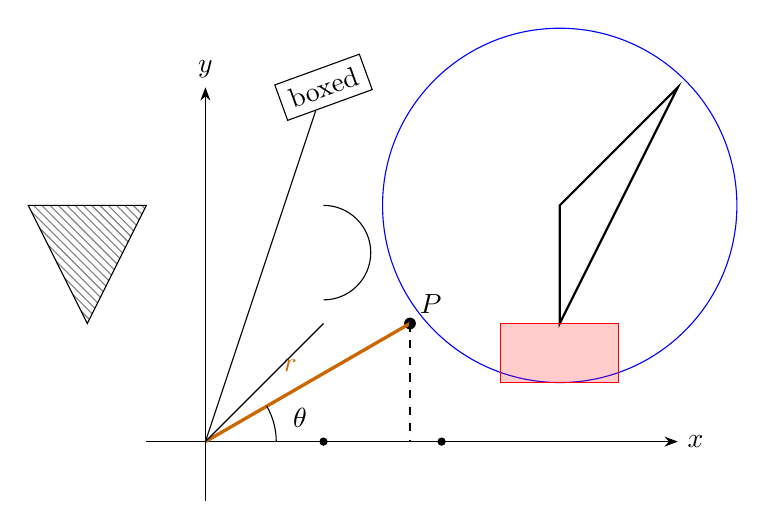
\begin{tikzpicture}[scale=1.5]
  % axes
  \draw[->,>=Stealth] (-0.5,0) -- (4,0) node[right] {$x$};
  \draw[->,>=Stealth] (0,-0.5) -- (0,3) node[above] {$y$};
  \coordinate (O) at (0,0);
  \coordinate (P) at (30:2);
  \node[circle, fill, inner sep=1.5pt] at (P) {};
  \node[above right] at (P) {$P$};
  \draw[accent, very thick] (O) -- (P) node[midway, above left] {$r$};
  \draw[dashed] (P) -- ($(P)!1!(P |- O)$);
  \draw (0.6,0) arc[start angle=0, end angle=30, radius=0.6];
  \node at (0.8,0.2) {$\theta$};
  \draw[blue] (3,2) circle (\R);
  \draw[thick] (3,2) -- +(1,1) -- ++(0,-1) -- cycle;
  \draw (1,2) arc (90:-90:0.4);
  \filldraw[red, fill opacity=0.2] (2.5,0.5) rectangle (3.5,1);
  \draw[pattern=north west lines, pattern color=gray] (-1,1) -- (-0.5,2) -- (-1.5,2) -- cycle;
  \node[draw, rotate=20] (box) at (1,3) {boxed};
  \draw (box) -- (O);
  \foreach \i in {1,2} \fill (\i,0) circle (1pt);
  \draw[decorate] (0,0) -- (1,1);
\end{tikzpicture}
\end{document}
